% ======================================================================
%  SIMC 2026 --- PRELIMINARY WORKING REPORT  \textperiodcentered{}  Questions 1, 2 & 3
%  Endeavour Track  \textperiodcentered{}  INTERNAL DRAFT --- full proofs, all details.
%
%  Source of all mathematical content:
%     notes/Note 26 May 2026.pdf      (Q1, parts a--b)
%     notes/Note 26 May 2026 (2).pdf  (Q1, parts a--e, g)
%     notes/task 2.pdf                (Q2, parts a--e)
%     src/task1/task1.ipynb           (Q1, parts f, h --- numerical validation)
%     src/task_3.ipynb                (Q3, parts a--g --- data analysis)
%
%  Every deviation from those notes (mistake fixed, gap filled, extra
%  added, elaboration) is logged in  changelog.md  in this folder.
%
%  Team:  K. Vishnu Kumar \textperiodcentered{} Adithya Kesan Jayakanth \textperiodcentered{} Adithya Anand
%  Date:  27 May 2026  (Q3 added; Q1/Q2 unchanged from the 26 May draft)
% ======================================================================

\documentclass[12pt,a4paper]{article}

\usepackage[a4paper, margin=2.0cm, headheight=14pt]{geometry}
\usepackage{mathptmx}                 % Times for text + math
\usepackage[T1]{fontenc}
\usepackage{amsmath,amssymb,amsthm,bm}
\usepackage{enumitem}
\usepackage{xcolor}
\usepackage{fancyhdr}
\usepackage{graphicx}
\usepackage{booktabs}
\usepackage[font=small,skip=3pt]{caption}
\usepackage[hidelinks]{hyperref}

% Q3 figures: space-free copies live in doc/FINAL/figs/; originals in data/output/TASK 3/.
\graphicspath{{../figs/}}

\linespread{1.10}
\setlength{\parskip}{5pt}
\setlength{\parindent}{0pt}

% --- header / footer --------------------------------------------------
\pagestyle{fancy}
\fancyhf{}
\fancyhead[L]{\small SIMC 2026 \textperiodcentered{} Preliminary Working Report (Q1, Q2 \& Q3)}
\fancyhead[R]{\small \thepage}
\fancyfoot[C]{\small Vishnu \textperiodcentered\ Adithya K.J. \textperiodcentered\ Adithya A. \quad\textbf{INTERNAL DRAFT --- NOT FOR SUBMISSION}}
\renewcommand{\headrulewidth}{0.4pt}

% --- review flags (mirrored in extras.md) -----------------------------
\newcommand{\miss}[1]{{\textbf{\textcolor{red}{[MISS: #1]}}}}
\newcommand{\fix}[1]{{\textbf{\textcolor{orange!85!black}{[CORRECTED: #1]}}}}
\newcommand{\extra}[1]{{\textbf{\textcolor{blue!80!black}{[EXTRA: #1]}}}}
\newcommand{\verified}[1]{{\textbf{\textcolor{green!45!black}{[VERIFIED: #1]}}}}

% --- proof environments -----------------------------------------------
\theoremstyle{definition}
\newtheorem*{claim}{Claim}
\newtheorem*{prop}{Proposition}
\DeclareMathOperator{\tr}{tr}

% --- notation shortcuts -----------------------------------------------
\newcommand{\R}{\mathbb{R}}
\newcommand{\Mx}{\mathbf{M}}
\newcommand{\Xb}{\mathbf{X}}
\newcommand{\vv}{\mathbf{v}}
\newcommand{\uu}{\mathbf{u}}
\newcommand{\xx}{\mathbf{x}}
\newcommand{\yy}{\mathbf{y}}
\newcommand{\pp}{\mathbf{p}}
\newcommand{\rr}{\mathbf{r}}
\newcommand{\zero}{\mathbf{0}}
\newcommand{\norm}[1]{\lVert #1 \rVert}
\newcommand{\T}{^{\!\top}}
% Q3 notation
\newcommand{\Xt}{\widetilde{\mathbf X}}
\newcommand{\xt}{\widetilde{\mathbf x}}
\newcommand{\Nt}{\widetilde{N}}
\newcommand{\Cc}{\mathbf{C}}
\newcommand{\Gg}{\mathbf{G}}
\newcommand{\nuv}{\boldsymbol{\nu}}

\title{\vspace{-1.6cm}\Huge\bfseries A Linear Algebra Guide to the\\Strange Life of High-Dimensional Data\\[0.4em]
\Large Preliminary Working Report --- Questions 1, 2 \& 3}
\author{K.\ Vishnu Kumar \and Adithya Kesan Jayakanth \and Adithya Anand}
\date{27 May 2026\\[0.3em]\small\itshape Internal draft: full proofs and all details.
Questions 1, 2 (analytical) and 3 (data analysis on \texttt{mystery\_matrix1.npy});
to be compressed into the 10-page submission. Extra detail is retained here for the oral defence.}

\begin{document}
\maketitle
\thispagestyle{fancy}

% =====================================================================
\section*{Scope and status of this draft}
\addcontentsline{toc}{section}{Scope and status}

This preliminary report contains the \emph{complete} worked solutions to all three
questions: \textbf{Question 1} (Linear Algebra of Markov Matrices) and \textbf{Question 2}
(The Power Method and Singular Value Decomposition), both purely analytical with every
proof written out in full, and \textbf{Question 3} (the data analysis on
\texttt{mystery\_matrix1.npy}), now added with its full computational pipeline, figures,
and propositions. It remains a working document, not the final submission: the generic
report scaffolding (literature, sensitivity studies) is kept light, and the whole will be
compressed to the 10-page cap for submission, with the surplus detail here reserved for the
oral defence.

\textbf{Status of Question 3.} Parts (a)--(h) are complete and reproduced from
\texttt{src/task\_3.ipynb} (every figure in this section is regenerated by that notebook and
stored under \texttt{data/output/TASK 3/}). Parts (a)--(e) consolidate the earlier
\texttt{doc/task 3 anand/Q3\_report.tex}; parts (f) (Gram-matrix clustering), (g) (the
covariance-vs-Gram comparison), and (h) (the taste-tester synthesis: how many unique samples) are
written up here for the first time. Question 1's
numerical-validation parts (f) and (h), flagged as misses in the 26 May draft, are now
implemented in \texttt{src/task1/task1.ipynb} and resolved below.

Coloured tags mark every place this document departs from, or extends, the team's
handwritten notes and the raw data. Each tag has a matching entry in \texttt{changelog.md}:
\begin{itemize}[leftmargin=1.4em, itemsep=1pt]
  \item \miss{\dots} --- a part of the problem not yet attempted in the notes.
  \item \fix{\dots} --- a mathematical error in the notes or a mismatch in the prompt, corrected here.
  \item \extra{\dots} --- content added beyond the notes (an elaboration or a missing explanation).
  \item \verified{\dots} --- a numerical or algebraic claim independently checked in code.
\end{itemize}

% =====================================================================
\section*{Notation and conventions}
\addcontentsline{toc}{section}{Notation and conventions}

\begin{tabular}{@{}p{0.20\linewidth}p{0.74\linewidth}@{}}
$\Mx,\ \Xb$ & matrices (bold uppercase). \\
$\vv,\uu,\xx,\pp$ & column vectors (bold lowercase). \\
$\Xb\T$ & transpose of $\Xb$, $(\Xb\T)_{ij}=\Xb_{ji}$. \\
$\lambda_i,\ \vv_i$ & eigenvalue / eigenvector pair, ordered $|\lambda_1|\ge|\lambda_2|\ge\cdots$. \\
$\sigma_i$ & singular value, $\sigma_i=\sqrt{\lambda_i}$. \\
$\norm{\xx}$ & Euclidean norm, $\norm{\xx}=\sqrt{\xx\T\xx}$. \\
$\Xb,\Xt$ & (Q3) design matrix (rows = samples), and its mean-centred form $\Xt_{ij}=\Xb_{ij}-\bar\Xb_j$. \\
$\Cc,\Gg$ & (Q3) covariance $\Cc=\tfrac1\Nt\Xt\T\Xt$ ($M\times M$); Gram $\Gg=\tfrac1\Nt\Xt\Xt\T$ ($\Nt\times\Nt$). \\
$\nuv_k$ & (Q3) $k$-th principal direction (eigenvector of $\Cc$); $\Nt$ = number of cleaned samples. \\
\end{tabular}

A set of vectors is \emph{orthonormal} if $\vv_i\T\vv_j=0$ for $i\ne j$ and
$\vv_i\T\vv_i=1$. We use the \textbf{spectral theorem} as a given: every real
symmetric matrix has real eigenvalues and an orthonormal basis of real
eigenvectors.

% =====================================================================
% =====================================================================
\section{Linear Algebra of Markov Matrices}

\textbf{Setup.} Two organism types have fractional populations
$p_1(t),p_2(t)$, evolving by $\pp(t+1)=\Mx\,\pp(t)$ with
\[
\pp(t)=\begin{pmatrix}p_1(t)\\ p_2(t)\end{pmatrix},
\qquad
\Mx=\begin{pmatrix}1-\varepsilon & 0\\[2pt] \varepsilon & 1\end{pmatrix},
\qquad \varepsilon\in(0,1)\ \text{fixed.}
\]
Componentwise this is
\begin{equation}\label{eq:update}
p_1(t+1)=(1-\varepsilon)\,p_1(t),\qquad
p_2(t+1)=\varepsilon\,p_1(t)+p_2(t).
\end{equation}
Each column of $\Mx$ sums to $1$ (it is \emph{column-stochastic}); a fraction
$\varepsilon$ of type-1 converts to type-2 each generation.

% ---------------------------------------------------------------------
\subsection{(a) Conservation}

\begin{claim}
$p_1(t)+p_2(t)$ is constant in $t$.
\end{claim}
\begin{proof}
Let $S(t)=p_1(t)+p_2(t)$. Adding the two equations in \eqref{eq:update},
\[
S(t+1)=p_1(t+1)+p_2(t+1)=(1-\varepsilon)p_1(t)+\bigl(\varepsilon\,p_1(t)+p_2(t)\bigr)
       = p_1(t)+p_2(t)=S(t).
\]
So $S(t+1)=S(t)$ for every $t$. By induction $S(t)=S(0)=p_1(0)+p_2(0)$, a
constant independent of $t$. \end{proof}

\textit{Equivalent one-line argument.} Because every column of $\Mx$ sums to
$1$, the row vector $\mathbf{1}\T=(1,1)$ satisfies $\mathbf{1}\T\Mx=\mathbf{1}\T$,
hence $\mathbf{1}\T\pp(t+1)=\mathbf{1}\T\Mx\,\pp(t)=\mathbf{1}\T\pp(t)$, i.e.\
$S(t+1)=S(t)$.

% ---------------------------------------------------------------------
\subsection{(b) Eigenspectrum}

The eigenvalues solve $\det(\Mx-\lambda \mathbf I)=0$:
\[
\det\!\begin{pmatrix}1-\varepsilon-\lambda & 0\\[2pt] \varepsilon & 1-\lambda\end{pmatrix}
=(1-\varepsilon-\lambda)(1-\lambda)=0
\quad\Longrightarrow\quad
\boxed{\lambda_1=1,\qquad \lambda_2=1-\varepsilon.}
\]
(The matrix is lower-triangular, so the eigenvalues are simply its diagonal
entries.) The eigenvectors come from $(\Mx-\lambda_i\mathbf I)\vv_i=\zero$.

\textit{For $\lambda_1=1$:}\quad
$\begin{pmatrix}-\varepsilon & 0\\ \varepsilon & 0\end{pmatrix}\!\begin{pmatrix}x\\ y\end{pmatrix}=\zero
\Rightarrow -\varepsilon x=0\Rightarrow x=0$, $y$ free. Take
$\displaystyle \vv_1=\begin{pmatrix}0\\1\end{pmatrix}.$

\textit{For $\lambda_2=1-\varepsilon$:}\quad
$\begin{pmatrix}0 & 0\\ \varepsilon & \varepsilon\end{pmatrix}\!\begin{pmatrix}x\\ y\end{pmatrix}=\zero
\Rightarrow \varepsilon(x+y)=0\Rightarrow y=-x$. Take
$\displaystyle \vv_2=\begin{pmatrix}1\\-1\end{pmatrix}.$

% ---------------------------------------------------------------------
\subsection{(c) Linear combination}

Assume $p_1(0)=\tfrac12$. Write
$\pp(0)=c_1\vv_1+c_2\vv_2=c_1\!\begin{pmatrix}0\\1\end{pmatrix}+c_2\!\begin{pmatrix}1\\-1\end{pmatrix}
=\begin{pmatrix}c_2\\ c_1-c_2\end{pmatrix}.$
Matching components,
\[
c_2=p_1(0)=\tfrac12,\qquad c_1-c_2=p_2(0)\ \Rightarrow\ c_1=p_2(0)+\tfrac12 .
\]
\fix{notes assumed $p_2(0)=\tfrac12$ without stating it.} If, as is natural for
fractional populations, the totals are normalised so that
$p_1(0)+p_2(0)=1$, then $p_2(0)=\tfrac12$ and $c_1=1$, giving
\[
\boxed{\ \pp(0)=\vv_1+\tfrac12\,\vv_2.\ }
\]
More generally $c_1=p_2(0)+\tfrac12$ and $c_2=\tfrac12$; note
$c_1=p_1(0)+p_2(0)=S(0)$, the conserved total from part (a).

% ---------------------------------------------------------------------
\subsection{(d) Eigenvectors make time evolution easy}

With $\pp(0)=c_1\vv_1+c_2\vv_2$, apply $\Mx$ repeatedly. Since
$\Mx\vv_i=\lambda_i\vv_i$, we have $\Mx^{t}\vv_i=\lambda_i^{\,t}\vv_i$, so
\[
\pp(t)=\Mx^{t}\pp(0)=c_1\lambda_1^{\,t}\vv_1+c_2\lambda_2^{\,t}\vv_2
\quad\Longrightarrow\quad
\boxed{\ \pp(t)=c_1\,\vv_1+c_2\,(1-\varepsilon)^{t}\,\vv_2.\ }
\]
The eigenbasis turns repeated matrix multiplication into scalar powers: each
mode evolves independently by its own factor $\lambda_i^{\,t}$.

% ---------------------------------------------------------------------
\subsection{(e) Long-time behaviour}

\textbf{(i)}~Because $\varepsilon\in(0,1)$ we have $0<1-\varepsilon<1$, so
$(1-\varepsilon)^{t}\to0$ as $t\to\infty$. Hence
\[
\pp(t)\ \xrightarrow{\ t\to\infty\ }\ c_1\vv_1,
\]
the eigenvector with the larger eigenvalue $\lambda_1=1>\lambda_2$.

\textbf{(ii)}~The structure of $\Mx$ explains this. The second column
$(0,1)\T$ means type-2 is \emph{absorbing}: nothing leaves it. Type-1 leaks
into type-2 at rate $\varepsilon$ every step and never receives anything back.
So all mass drains into type-2. Quantitatively the limit is
\[
c_1\vv_1=\begin{pmatrix}0\\ c_1\end{pmatrix}
=\begin{pmatrix}0\\ p_1(0)+p_2(0)\end{pmatrix},
\]
i.e.\ the entire conserved population $S(0)$ ends up as type-2. The eigenvalue
$\lambda_1=1$ carries the conserved steady state, while $\lambda_2=1-\varepsilon<1$
governs the decaying transient.

% ---------------------------------------------------------------------
\subsection{(f) Validation}

\miss{flagged as not-attempted in the 26 May notes;} \verified{now implemented in
\texttt{src/task1/task1.ipynb}.} The closed form
$\pp(t)=c_1\vv_1+c_2(1-\varepsilon)^t\vv_2$ is checked against a direct numerical
iteration of $\pp(t+1)=\Mx\pp(t)$ from $\pp(0)=(\tfrac12,\tfrac12)$ with
$\varepsilon=0.1$ over $T=100$ generations. The two tracks agree to machine
precision ($\max_t\norm{\pp_{\text{num}}(t)-\pp_{\text{closed}}(t)}\approx10^{-16}$),
and $\pp(t)\to(0,1)$ as predicted by part (e). Figure~\ref{fig:t1f} shows the
linear-scale convergence (Panel A) and the semi-log decay of $p_1(t)$ overlaid on
$\tfrac12(1-\varepsilon)^t$, a straight line confirming the geometric rate (Panel B).

\begin{figure}[h]\centering
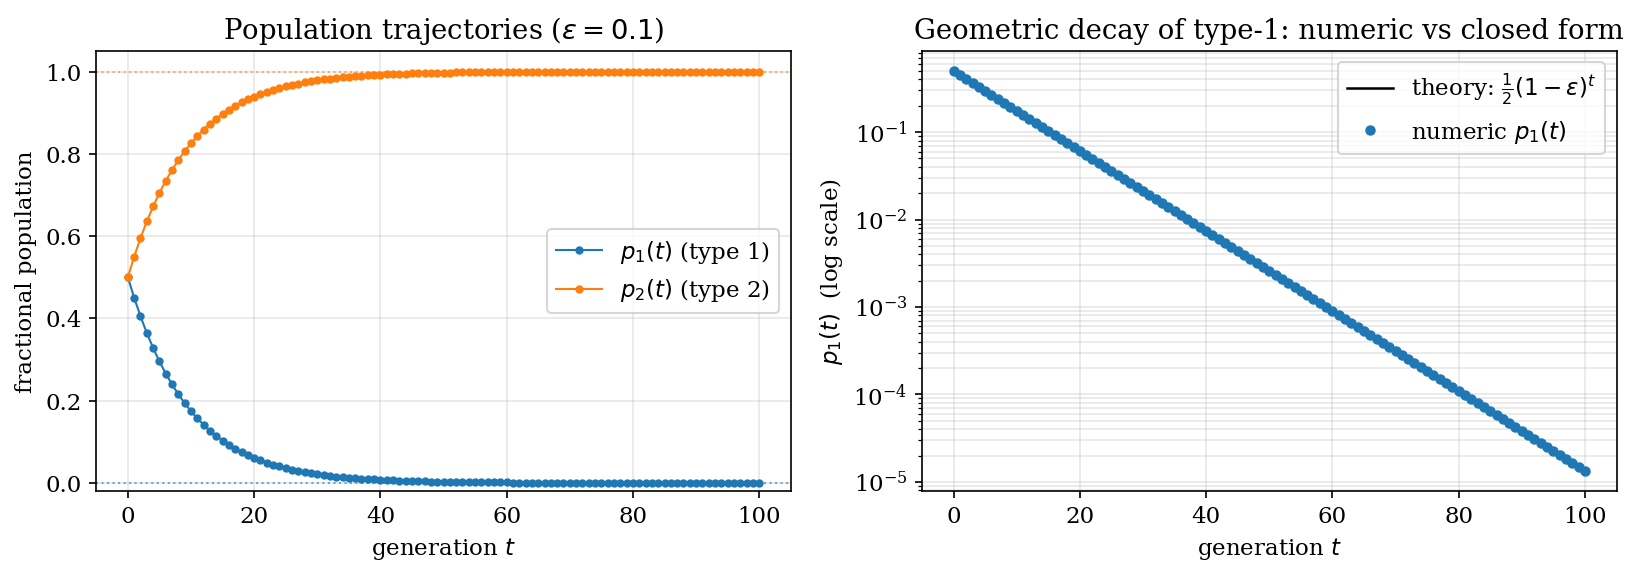
\includegraphics[width=0.86\linewidth]{task1f_trajectories.png}
\caption{(1f) Direct iteration vs the closed form for constant $\varepsilon=0.1$.
Panel A: $p_1,p_2$ converge to $(0,1)$. Panel B: $p_1(t)$ (dots) lies exactly on
$\tfrac12(1-\varepsilon)^t$ (line) on a semi-log axis --- geometric decay at rate
$1-\varepsilon$, validating parts (d) and (e).}\label{fig:t1f}
\end{figure}

% ---------------------------------------------------------------------
\subsection{(g) Time-varying conversion rate}

Now $\varepsilon(t)=\varepsilon_0\,e^{-t/t_0}$ with $\varepsilon_0,t_0>0$, so the
update matrix changes each step:
$\Mx(t)=\bigl(\begin{smallmatrix}1-\varepsilon(t) & 0\\ \varepsilon(t) & 1\end{smallmatrix}\bigr)$.

\fix{the notes wrote $\pp(t)=1^{t}c_1+\bigl(1-\varepsilon(t)\bigr)^{t}c_2$, which is
not correct for a time-varying rate.} The key observation is that the
eigenvectors $\vv_1=(0,1)\T$ and $\vv_2=(1,-1)\T$ \emph{do not depend on
$\varepsilon$}, so they are shared by \emph{every} matrix $\Mx(t)$:
\[
\Mx(t)\,\vv_1=1\cdot\vv_1,\qquad \Mx(t)\,\vv_2=\bigl(1-\varepsilon(t)\bigr)\vv_2 .
\]
The state is the ordered product $\pp(t)=\Mx(t-1)\Mx(t-2)\cdots\Mx(0)\,\pp(0)$.
Acting on $\pp(0)=c_1\vv_1+c_2\vv_2$, the $\vv_1$ mode is multiplied by $1$ at
every step, while the $\vv_2$ mode picks up one factor $\bigl(1-\varepsilon(s)\bigr)$
per step. Therefore
\[
\boxed{\ \pp(t)=c_1\,\vv_1+c_2\Bigl[\textstyle\prod_{s=0}^{t-1}\bigl(1-\varepsilon_0 e^{-s/t_0}\bigr)\Bigr]\vv_2.\ }
\]
So the constant-rate factor $(1-\varepsilon)^{t}$ of part (d) is replaced by the
\textbf{product} $\prod_{s=0}^{t-1}\bigl(1-\varepsilon(s)\bigr)$, not by
$\bigl(1-\varepsilon(t)\bigr)^{t}$.

\extra{qualitative consequence (beyond the notes).} Since
$\sum_{s\ge0}\varepsilon_0 e^{-s/t_0}<\infty$, the infinite product converges to a
\emph{strictly positive} limit $\Pi_\infty=\prod_{s=0}^{\infty}\bigl(1-\varepsilon_0 e^{-s/t_0}\bigr)$.
Unlike the constant-$\varepsilon$ case, the $\vv_2$ transient does \emph{not}
decay to zero: the conversion ``switches off'' as $\varepsilon(t)\to0$, freezing a
residual amount $c_2\Pi_\infty$ in the $\vv_2$ direction. The system therefore
settles at $\pp(\infty)=c_1\vv_1+c_2\Pi_\infty\vv_2$, i.e.\ type-1 is
\emph{not} fully depleted.

% ---------------------------------------------------------------------
\subsection{(h) Validate again}

\miss{flagged as not-attempted in the 26 May notes;} \verified{now implemented in
\texttt{src/task1/task1.ipynb}.} The corrected \emph{product} formula for part (g) is
validated the same way as (f): we iterate $\pp(t+1)=\Mx(t)\pp(t)$ with
$\varepsilon(t)=\varepsilon_0 e^{-t/t_0}$ ($\varepsilon_0=0.5,\ t_0=10$) and compare
against $c_1\vv_1+c_2\prod_{s<t}(1-\varepsilon(s))\,\vv_2$. The tracks again agree to
machine precision, and --- unlike the constant-rate case --- the $\vv_2$ transient
\emph{freezes} at a strictly positive residual $c_2\Pi_\infty$ rather than decaying to
zero, confirming the qualitative claim of part (g): type-1 is not fully depleted.
Figure~\ref{fig:t1h} overlays the decaying-rate trajectory (solid) on the constant-rate
reference (faded) to make the frozen residual visible.

\begin{figure}[h]\centering
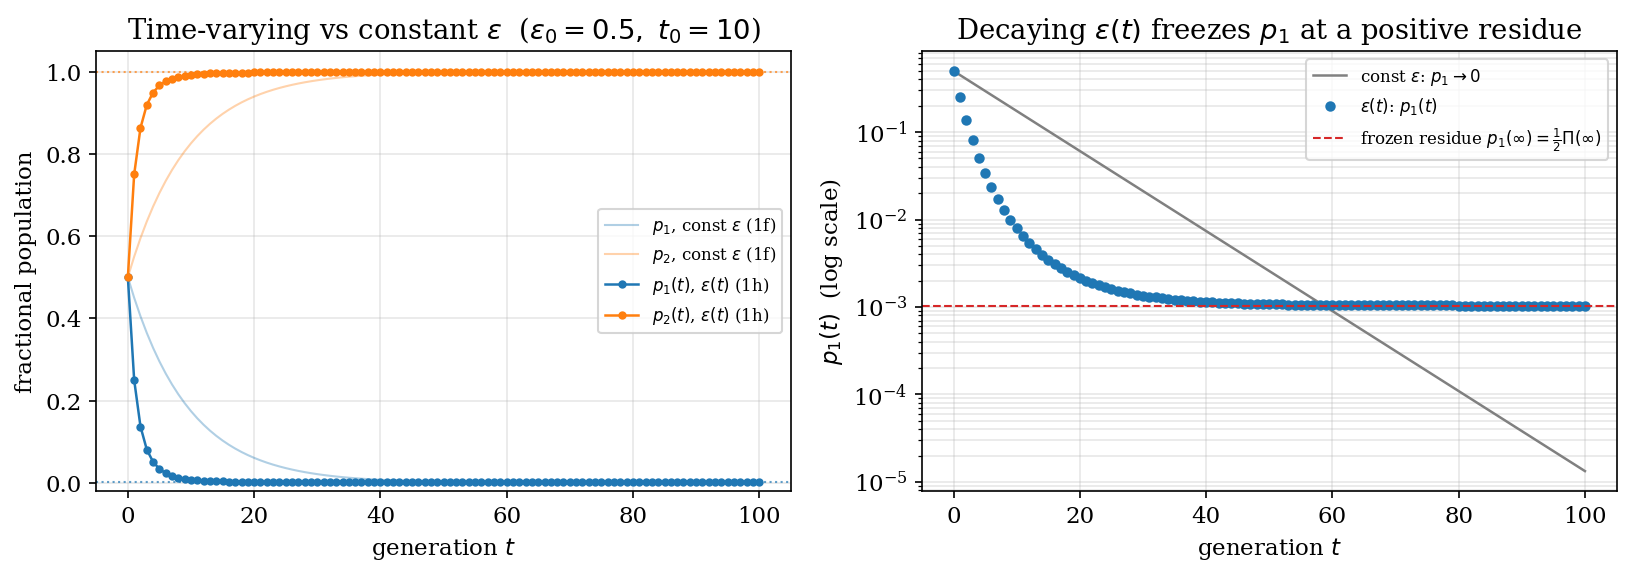
\includegraphics[width=0.86\linewidth]{task1h_trajectories.png}
\caption{(1h) Time-varying $\varepsilon(t)=\varepsilon_0 e^{-t/t_0}$ (solid) vs constant
$\varepsilon$ (faded). The conversion ``switches off'' as $\varepsilon(t)\to0$, so $p_1$
settles at a positive plateau $c_2\Pi_\infty>0$ instead of draining to zero --- validating
the product formula and the residual claim of part (g).}\label{fig:t1h}
\end{figure}

% =====================================================================
% =====================================================================
\section{The Power Method and Singular Value Decomposition}

\textbf{Setup.} $\Xb$ is a symmetric $n\times n$ matrix with eigenvalues
$|\lambda_1|>|\lambda_2|\ge\cdots\ge|\lambda_n|$ and an orthonormal eigenbasis
$\vv_1,\dots,\vv_n$. The Power Method starts from a unit vector $\xx_0$ and
iterates
\begin{equation}\label{eq:power}
\xx_{k+1}=\frac{\Xb\,\xx_k}{\norm{\Xb\,\xx_k}},\qquad k=0,1,2,\dots
\end{equation}

% ---------------------------------------------------------------------
\subsection{(a) The Power Method converges}

\begin{claim}
If $\xx_0$ has a nonzero component along $\vv_1$, then $\xx_k\to\pm\vv_1$.
\end{claim}
\begin{proof}
Normalisation in \eqref{eq:power} only rescales, so $\xx_k$ has the same
\emph{direction} as the unnormalised iterate
$\yy_k:=\Xb^{k}\xx_0$. Expand $\xx_0$ in the orthonormal eigenbasis,
\[
\xx_0=\sum_{i=1}^{n} a_i\vv_i,\qquad a_i=\xx_0\T\vv_i,\qquad a_1\ne0 .
\]
Since $\Xb^{k}\vv_i=\lambda_i^{k}\vv_i$,
\[
\yy_k=\Xb^{k}\xx_0=\sum_{i=1}^{n} a_i\lambda_i^{k}\vv_i
      =\underbrace{a_1\lambda_1^{k}\vv_1}_{\text{parallel to }\vv_1}
      +\underbrace{\sum_{i=2}^{n} a_i\lambda_i^{k}\vv_i}_{=\ \rr_k\ \text{(residual)}} .
\]
By orthonormality the residual length is
$\norm{\rr_k}^2=\sum_{i=2}^{n} a_i^2\lambda_i^{2k}$. Measure the residual
relative to the parallel part:
\[
\rho_k:=\frac{\norm{\rr_k}}{|a_1|\,|\lambda_1|^{k}}
       =\frac{1}{|a_1|}\sqrt{\sum_{i=2}^{n} a_i^2\Bigl(\tfrac{\lambda_i}{\lambda_1}\Bigr)^{2k}} .
\]
For every $i\ge2$ we have $|\lambda_i/\lambda_1|<1$, so each term
$(\lambda_i/\lambda_1)^{2k}\to0$ and hence $\rho_k\to0$. Thus $\yy_k$ aligns
with $\vv_1$, and after normalisation $\xx_k\to\pm\vv_1$ (the sign tracks
$\operatorname{sign}(a_1\lambda_1^{k})$). \end{proof}

% ---------------------------------------------------------------------
\subsection{(b) Convergence rate and the spectral gap}

\begin{claim}
The residual ratio shrinks each step by at least $|\lambda_2/\lambda_1|$:
$\ \rho_{k+1}/\rho_k\le |\lambda_2/\lambda_1|$.
\end{claim}
\begin{proof}
From the definition of $\rho_k$,
\[
\frac{\rho_{k+1}}{\rho_k}
=\frac{1}{|\lambda_1|}\,
\sqrt{\frac{\sum_{i\ge2} a_i^2\lambda_i^{2k+2}}{\sum_{i\ge2} a_i^2\lambda_i^{2k}}}\, .
\]
Put $\omega_i:=a_i^2\lambda_i^{2k}\ge0$. The fraction under the root is the
weighted average $\bigl(\sum_{i\ge2}\omega_i\lambda_i^{2}\bigr)\big/\bigl(\sum_{i\ge2}\omega_i\bigr)$
of the numbers $\{\lambda_i^2:i\ge2\}$, which cannot exceed their maximum
$\lambda_2^{2}$. Therefore
\[
\frac{\rho_{k+1}}{\rho_k}\le\frac{1}{|\lambda_1|}\sqrt{\lambda_2^{2}}
=\Bigl|\tfrac{\lambda_2}{\lambda_1}\Bigr|<1 .
\]
\end{proof}
Convergence is therefore \textbf{geometric} with rate $|\lambda_2/\lambda_1|$.
The quantity $|\lambda_1|-|\lambda_2|$ (equivalently the ratio
$|\lambda_2/\lambda_1|$) is the \textbf{spectral gap}: a large gap means fast,
robust convergence; a small gap means slow convergence vulnerable to noise.

% ---------------------------------------------------------------------
\subsection{(c) When the spectral gap closes}

\textbf{(i)}~Take $\displaystyle \Xb=\begin{pmatrix}1&0\\0&-1\end{pmatrix}$,
with $\lambda_1=1,\ \lambda_2=-1$, so $|\lambda_1|=|\lambda_2|=1$ (no gap).
For a generic start $\xx_0=(a,b)$ with $a,b\ne0$,
\[
\xx_1=\Xb\xx_0=\begin{pmatrix}a\\-b\end{pmatrix},\quad
\xx_2=\begin{pmatrix}a\\ b\end{pmatrix},\quad
\xx_3=\begin{pmatrix}a\\-b\end{pmatrix},\ \dots
\quad\Longrightarrow\quad
\Xb^{k}\xx_0=\begin{pmatrix}a\\ (-1)^{k}b\end{pmatrix}.
\]
The norm $\sqrt{a^2+b^2}$ is preserved, so after normalisation $\xx_k$
oscillates forever between the two distinct directions
$(a,b)$ and $(a,-b)$ and never converges to a single vector.

\textbf{(ii)}~\extra{explanation not written in the notes.} A vanishing gap is
a \emph{structural} obstruction, not merely slow convergence. The Power Method
works by amplifying each eigencomponent by its own factor $\lambda_i^{k}$; the
top direction wins only because $|\lambda_1|>|\lambda_i|$. When
$|\lambda_1|=|\lambda_2|$ the leading components are amplified by the
\emph{same} factor every step, so their relative weights never change: there is
no selection mechanism. The iterate keeps whatever mixture it started with --
oscillating (as above, when the eigenvalues differ in sign) or, in the
degenerate case $\lambda_1=\lambda_2$, converging to an essentially arbitrary
vector of the eigenspace rather than to a unique eigenvector. In the rate of
part (b), $|\lambda_2/\lambda_1|=1$, so $\rho_k$ does not decay at all.

\textbf{(iii)}~\extra{explanation not written in the notes.} When
$|\lambda_2/\lambda_1|$ is close to (but below) $1$, two problems compound.
First, the number of iterations needed scales like
$1/\bigl(1-|\lambda_2/\lambda_1|\bigr)$, which blows up. Second, each step of
double-precision arithmetic injects rounding error of order $10^{-16}$ into
\emph{all} directions, including $\vv_2$. The useful per-step separation
between $\vv_1$ and $\vv_2$ is only $\propto |\lambda_2/\lambda_1|^{k}$; once that
signal falls to the level of the accumulated noise, the computed vector drifts
within the near-degenerate $\{\vv_1,\vv_2\}$ subspace and the ordering of the
two eigenvalues becomes numerically ambiguous.

% ---------------------------------------------------------------------
\subsection{(d) The two symmetric matrices $\Xb\T\Xb$ and $\Xb\Xb\T$}

Let $\Xb$ be a general (rectangular) $m\times n$ matrix.

\textbf{(i) Symmetric and positive semi-definite.}
\[
(\Xb\T\Xb)\T=\Xb\T(\Xb\T)\T=\Xb\T\Xb,\qquad
(\Xb\Xb\T)\T=\Xb\Xb\T,
\]
so both products are symmetric. For positive semi-definiteness, take any real
vector $\mathbf w$ of the appropriate size:
\[
\mathbf w\T(\Xb\T\Xb)\mathbf w=(\Xb\mathbf w)\T(\Xb\mathbf w)=\norm{\Xb\mathbf w}^2\ge0,
\qquad
\mathbf w\T(\Xb\Xb\T)\mathbf w=\norm{\Xb\T\mathbf w}^2\ge0 .
\]
\fix{the notes wrote $\norm{\Xb\T\mathbf w}^2$ for the $\Xb\T\Xb$ case; the correct
quantity there is $\norm{\Xb\mathbf w}^2$.} Being symmetric (real eigenvalues, by
the spectral theorem) and PSD ($\mathbf w\T A\mathbf w\ge0\Rightarrow$ eigenvalues
$\ge0$), both matrices have \emph{real, non-negative} eigenvalues. Hence
$\sigma_i:=\sqrt{\lambda_i}$ is well defined.

\textbf{(ii) Same nonzero eigenvalues.}
Suppose $\Xb\T\Xb\,\vv=\lambda\vv$ with $\lambda\ne0$ (so $\vv\ne\zero$).
Left-multiplying by $\Xb$,
\[
\Xb(\Xb\T\Xb\,\vv)=\lambda\,\Xb\vv
\quad\Longrightarrow\quad
(\Xb\Xb\T)(\Xb\vv)=\lambda\,(\Xb\vv).
\]
Moreover $\Xb\vv\ne\zero$, since $\Xb\vv=\zero$ would give
$\Xb\T\Xb\vv=\zero=\lambda\vv$, forcing $\lambda=0$. Thus $\Xb\vv$ is an
eigenvector of $\Xb\Xb\T$ with the same eigenvalue $\lambda$. The same argument
with $\Xb\T$ shows every nonzero eigenvalue of $\Xb\Xb\T$ is an eigenvalue of
$\Xb\T\Xb$. Hence $\Xb\T\Xb$ and $\Xb\Xb\T$ have \emph{identical nonzero
eigenvalues}, the shared values being $\sigma_i^{2}$.

% ---------------------------------------------------------------------
\subsection{(e) Power Method for the SVD: algorithm and worked example}

\textbf{(i) Algorithm (language-agnostic pseudocode).} Input: an
$N\times M$ matrix $\Xb$. Output: the top singular triplet
$\sigma_1,\vv_1,\uu_1$.
\begin{enumerate}[leftmargin=2.0em, itemsep=1pt, label=\arabic*.]
  \item \textbf{Form the smaller symmetric matrix.}
        If $N\ge M$, set $A\leftarrow\Xb\T\Xb$ (size $M\times M$);
        otherwise set $A\leftarrow\Xb\Xb\T$ (size $N\times N$).
  \item \textbf{Power iteration on $A$.} Choose a random unit vector $\xx$.
        Repeat $\xx\leftarrow A\xx/\norm{A\xx}$ until
        $\norm{A\xx/\norm{A\xx}-\xx}<\text{tol}$ (or a maximum iteration count).
  \item \textbf{Read off the singular value.}
        $\lambda_1\leftarrow \xx\T A\,\xx$ (Rayleigh quotient);
        $\sigma_1\leftarrow\sqrt{\lambda_1}$.
  \item \textbf{Recover the companion vector.}
        If $A=\Xb\T\Xb$: set $\vv_1\leftarrow\xx\in\R^{M}$ and
        $\uu_1\leftarrow \Xb\vv_1/\sigma_1\in\R^{N}$.
        If $A=\Xb\Xb\T$: set $\uu_1\leftarrow\xx\in\R^{N}$ and
        $\vv_1\leftarrow \Xb\T\uu_1/\sigma_1\in\R^{M}$.
  \item \textbf{Return} $\sigma_1,\vv_1,\uu_1$.
\end{enumerate}
\textit{Choice of matrix.} $A$ is square of size $\min(N,M)$. When $N\ll M$ the
$N\times N$ matrix $\Xb\Xb\T$ is far cheaper to store and to multiply, and when
$M\ll N$ the $M\times M$ matrix $\Xb\T\Xb$ is cheaper -- always pick the smaller.
\fix{the pseudocode text in the notes labelled this rule backwards (``if
$N\gg M$ compute $\Xb\Xb\T$''), although the stated reason and the worked
example below both use the smaller matrix. The consistent rule is given above.}

\textbf{(ii) Worked example by hand.}
\[
\Xb=\begin{pmatrix}1&0\\0&1\\1&1\end{pmatrix}\quad(N=3,\ M=2).
\]
Here $N>M$, so use the $2\times2$ matrix
\[
\Xb\T\Xb=\begin{pmatrix}1&0&1\\0&1&1\end{pmatrix}
\begin{pmatrix}1&0\\0&1\\1&1\end{pmatrix}
=\begin{pmatrix}2&1\\1&2\end{pmatrix}.
\]
\emph{Eigenvalues:}\quad
$\det\!\begin{pmatrix}2-\lambda&1\\1&2-\lambda\end{pmatrix}=(2-\lambda)^2-1
=\lambda^2-4\lambda+3=(\lambda-1)(\lambda-3)=0,$
so $\lambda=1$ or $\lambda=3$; the dominant one is $\lambda_1=3$.

\emph{Eigenvector for $\lambda_1=3$:}\quad $(2-3)x+y=0\Rightarrow y=x$, giving the
unit vector $\displaystyle\vv_1=\tfrac{1}{\sqrt2}\begin{pmatrix}1\\1\end{pmatrix}.$

\emph{Singular value:}\quad $\sigma_1=\sqrt{\lambda_1}=\sqrt3.$

\emph{Left singular vector:}\quad
\[
\uu_1=\frac{\Xb\vv_1}{\sigma_1}
=\frac{1}{\sqrt3}\cdot\frac{1}{\sqrt2}\begin{pmatrix}1&0\\0&1\\1&1\end{pmatrix}\!\begin{pmatrix}1\\1\end{pmatrix}
=\frac{1}{\sqrt6}\begin{pmatrix}1\\1\\2\end{pmatrix}.
\]

\emph{Verification.}
\[
\Xb\vv_1=\tfrac{1}{\sqrt2}\begin{pmatrix}1\\1\\2\end{pmatrix},
\qquad
\sigma_1\uu_1=\sqrt3\cdot\tfrac{1}{\sqrt6}\begin{pmatrix}1\\1\\2\end{pmatrix}
=\tfrac{1}{\sqrt2}\begin{pmatrix}1\\1\\2\end{pmatrix}
\ \Rightarrow\ \Xb\vv_1=\sigma_1\uu_1.\ \checkmark
\]
\[
\Xb\T\uu_1=\tfrac{1}{\sqrt6}\begin{pmatrix}1&0&1\\0&1&1\end{pmatrix}\!\begin{pmatrix}1\\1\\2\end{pmatrix}
=\tfrac{1}{\sqrt6}\begin{pmatrix}3\\3\end{pmatrix}
=\tfrac{3}{\sqrt6}\begin{pmatrix}1\\1\end{pmatrix},
\qquad
\sigma_1\vv_1=\sqrt3\cdot\tfrac{1}{\sqrt2}\begin{pmatrix}1\\1\end{pmatrix}
=\sqrt{\tfrac32}\begin{pmatrix}1\\1\end{pmatrix},
\]
and $\tfrac{3}{\sqrt6}=\sqrt{\tfrac32}$, so $\Xb\T\uu_1=\sigma_1\vv_1.$ \checkmark
Both SVD relations hold, confirming $(\sigma_1,\vv_1,\uu_1)$.

% =====================================================================
% =====================================================================
\section{Design, Covariance and Gram Matrices: PCA of a Spectroscopy Dataset}

\textbf{Setup.} We are given \texttt{mystery\_matrix1.npy}, a set of infrared
absorbance spectra. The design matrix $\Xb\in\R^{N\times M}$ has rows $=$ samples
(vials) and columns $=$ features (frequency channels); $\Xb_{ij}$ is the absorbance of
vial $i$ at frequency $j$.
\fix{the prompt quotes $M=3041$ features, but the supplied array has $3401$ columns (a
digit transposition); the file is also stored \emph{transposed}, as $3401\times1000$.}
We key off the axis of length $1000$ (the samples), transpose once so rows index samples,
and use the array's true $M=3401$ throughout, flagging the discrepancy rather than
hard-coding either number. Every figure in this section is regenerated by
\texttt{src/task\_3.ipynb}.

% ---------------------------------------------------------------------
\subsection{(a) Cleaning the design matrix}

\textbf{(i) Empty vials.} An empty vial records only background noise: small, flat, hence
small Euclidean norm $\norm{\xx_i}=(\sum_j \Xb_{ij}^2)^{1/2}$. Sorting the $1000$ row norms
reveals a clean bimodal gap --- $40$ vials sit at $\norm{\xx}\approx1.6$, then a void until
the bulk begins at $\norm{\xx}\approx4.3$. We threshold at the gap midpoint; the count is
invariant for any cutoff in $[2.0,4.0]$, which is the evidence that the cut is principled,
not arbitrary. This flags exactly $T=40$ empties (rows $960$--$999$).
\verified{the removed group is flat ($50.2\%$ exact zeros, since background noise clipped
at zero is $0$ with probability $\approx\tfrac12$) while the retained group is peaked
($24.5\%$ zeros).}

\textbf{(ii) A second error.}
\extra{beyond the empty vials, the row-norm distribution shows a second anomalous group not
mentioned in the prompt:} $36$ vials at $\norm{\xx}\approx8.9$ (rows $924$--$959$), detached
from the bulk by a gap $\approx5\times$ wider than any internal gap. We retain a vial iff
$\tau_{\mathrm{lo}}\le\norm{\xx_i}\le\tau_{\mathrm{hi}}$ via a Boolean keep-mask
(non-destructive, composable, index-preserving), leaving $\Nt=924$ spectra.
\verified{these $36$ form one isolated cluster: in the top-4 PC space their cluster radius
is $\approx 1$ while the gap to the nearest other vial is many times larger, and removing
them drops the cluster count by exactly one, leaving every other group untouched
(Figure~\ref{fig:q3aii}). The decision is therefore clean and reversible.}

\begin{figure}[h]\centering

\includegraphics[width=0.62\linewidth]{q3a_part_i.png}
\caption{(3a-i) Row-norm distribution of the $1000$ measurements: $40$ empty vials isolated
below the gap (threshold dashed).}\label{fig:q3ai}
\end{figure}

\begin{figure}[h]\centering

\includegraphics[width=0.52\linewidth]{q3a_part_ii_clusters.png}
\caption{(3a-ii) The $36$ high-norm vials (red) form one well-separated cluster in the
top-2 PC plane; removing them deletes exactly one cluster.}\label{fig:q3aii}
\end{figure}

% ---------------------------------------------------------------------
\subsection{(b) Per-feature variance and the covariance matrix}

Mean-centring, $\Xt_{ij}=\Xb_{ij}-\bar\Xb_j$ with $\bar\Xb_j=\tfrac1\Nt\sum_i \Xb_{ij}$,
removes the shared mean spectrum so the analysis describes how samples \emph{differ}. The
covariance matrix is $\Cc=\tfrac1\Nt\Xt\T\Xt\in\R^{M\times M}$.

\begin{prop}
$\Cc$ is symmetric and $\Cc_{jj}=\tfrac1\Nt\sum_k\Xt_{kj}^2=\mathrm{Var}_j$, the variance of
feature $j$.
\end{prop}
\begin{proof}
$\Cc\T=\tfrac1\Nt(\Xt\T\Xt)\T=\Cc$; setting the row/column indices equal and using zero
column-means gives the variance. \end{proof}

\begin{prop}
$\tr\Cc=\sum_j\mathrm{Var}_j$ (total variance) is invariant under orthogonal change of basis
and equals $\sum_i\lambda_i$.
\end{prop}
\begin{proof}
$\tr(\mathbf Q\T\Cc\mathbf Q)=\tr(\Cc\mathbf Q\mathbf Q\T)=\tr\Cc$ for $\mathbf Q\T\mathbf Q=\mathbf I$;
diagonalising $\Cc=\mathbf Q\Lambda\mathbf Q\T$ gives $\tr\Cc=\sum_i\lambda_i$. \end{proof}

\verified{empirically $\tr\Cc\approx7.90$, and $\sum_i\lambda_i$ matches it to rounding
(a consistency check on the eigendecomposition below).} \textbf{(i)} the single
largest-variance feature is $j^\star=910$ with $\Cc_{j^\star j^\star}\approx0.0199$.
\textbf{(ii)+(iii)} the variance is not spread evenly: it concentrates in a few narrow
molecular bands separated by broad flat baseline (Figure~\ref{fig:q3b}). The data is
therefore highly redundant and effectively low-dimensional --- exactly the structure PCA
exploits in part (c).

\begin{figure}[h]\centering

\includegraphics[width=0.80\linewidth]{q3b_variance.png}
\caption{(3b) Per-feature variance $\Cc_{jj}$ across the $3401$ frequencies; the maximum at
$j^\star=910$ is dashed. Variance lives in a few bands, not the baseline.}\label{fig:q3b}
\end{figure}

% ---------------------------------------------------------------------
\subsection{(c) The eigenspectrum (PCA)}

\begin{prop}
For a unit vector $\mathbf w$, the variance of the data along $\mathbf w$ is
$\mathbf w\T\Cc\mathbf w$; if $\Cc\nuv=\lambda\nuv$ with $\norm{\nuv}=1$ then
$\nuv\T\Cc\nuv=\lambda$. Moreover $\Cc$ is PSD, so every $\lambda_i\ge0$.
\end{prop}
\begin{proof}
The projections $z_i=\xt_i\!\cdot\mathbf w$ have variance $\tfrac1\Nt\sum_i z_i^2=
\mathbf w\T\Cc\mathbf w=\tfrac1\Nt\norm{\Xt\mathbf w}^2\ge0$; substituting an eigenvector gives
$\lambda=\nuv\T\Cc\nuv\ge0$. \end{proof}

By the spectral theorem $\Cc$ has real eigenvalues and an orthonormal eigenbasis. We use
\texttt{numpy.linalg.eigh} (the symmetric solver: real eigenvalues, orthonormal
eigenvectors, faster and stabler than \texttt{eig}), sort decreasingly, and clip
rounding-level negatives to $0$.

\begin{table}[h]\centering\small
\begin{tabular}{lccccccccc}
\toprule
$k$ & 1 & 2 & 3 & 4 & 5 & 6 & 7 & 8 & 9\\
$\lambda_k$ & 2.492 & 0.705 & 0.590 & 0.254 & 0.123 & 0.105 & 0.078 & 0.039 & 0.0093\\
\bottomrule
\end{tabular}
\caption{Leading eigenvalues. The drop $\lambda_8/\lambda_9\approx4.1$ is the largest in the
spectrum.}\label{tab:q3eig}
\end{table}

\textbf{(i)} the dominance ratio is $\lambda_1/\lambda_2\approx3.53$, and $\lambda_1$ alone
explains $\approx31\%$ of the total variance. \textbf{(iv)} a large ratio means one
direction dominates the sample-to-sample variation: the data has a strong principal axis and
is effectively low-dimensional (and, echoing Q2, the wide spectral gap would make the Power
Method converge quickly here). \textbf{(iii) the elbow.} The elbow is the largest
multiplicative drop between consecutive eigenvalues (a ratio, because the signal/noise
boundary is multiplicative on the log scale): $\lambda_8/\lambda_9\approx4.1$ gives
$k^\star=8$. On the log plot (Figure~\ref{fig:q3c}) the first eight eigenvalues fall steeply,
then flatten into a noise floor of $\approx900$ near-equal values. This matches the
$\sim10$ dominant molecules referenced in part (h).

\extra{the ``keep $95\%$ of variance'' rule is misleading here and the elbow is the honest
measure.} The $8$ signal components explain only $\approx55\%$ of the variance; reaching
$95\%$ needs $k=667$ components (Table~\ref{tab:q3cum}), because the noise floor, though
individually tiny, is spread over hundreds of dimensions that sum to a large fraction. A
$95\%$ cut would pull in $\approx660$ noise directions and badly overstate the
dimensionality.

\begin{table}[h]\centering\small
\begin{tabular}{lccccc}
\toprule
cumulative variance & $50\%$ & $80\%$ & $90\%$ & $95\%$ & $99\%$\\
components $k$ & 4 & 309 & 516 & 667 & 850\\
\bottomrule
\end{tabular}
\caption{Components needed to reach each variance threshold: contrast the $8$ signal
components ($\approx55\%$) with the $667$ required for $95\%$.}\label{tab:q3cum}
\end{table}

\begin{figure}[h]\centering

\includegraphics[width=0.82\linewidth]{q3c_spectrum.png}\\[2pt]

\includegraphics[width=0.66\linewidth]{q3c_cvarr.png}
\caption{(3c) Top: eigenvalue spectrum (linear and log) with the sharp elbow at $k^\star=8$.
Bottom: cumulative variance --- $8$ components reach only $\approx55\%$; $95\%$ needs
$\approx667$.}\label{fig:q3c}
\end{figure}

% ---------------------------------------------------------------------
\subsection{(d) The leading eigenvector}

$\nuv_1\in\R^M$ (feature space) gives each frequency a \emph{loading}; the \emph{scores}
$z_i=\xt_i\!\cdot\nuv_1$ are the maximally-spread one-dimensional summaries. Eigenvectors are
sign-ambiguous, so we fix the largest loading positive. \textbf{(i)} the loadings are
supported on two narrow bands ($j\approx900$--$960$ and $3150$--$3260$) with $\approx27\%$
negative entries, so $\nuv_1$ is a \emph{contrast} direction (the balance of absorption
between bands), not overall intensity. \textbf{(ii)} with cosine similarity
$\cos(\mathbf a,\mathbf b)=\frac{\mathbf a\cdot\mathbf b}{\norm{\mathbf a}\norm{\mathbf b}}$,
$\nuv_1$ matches a \emph{centred} spectrum at $\cos\approx0.92$, but only $0.67$ against the
raw spectrum and $0.03$ against the mean spectrum. Living in the centred space by
construction, $\nuv_1$ is $\approx$orthogonal to the shared mean and is a
\emph{difference-spectrum} (Figure~\ref{fig:q3d}) --- it looks like a real measurement's
deviation from average, not the average itself. This is exactly what mean-centring buys, and
it echoes Q1's dominant-eigenvector steady state.

\begin{figure}[h]\centering

\includegraphics[width=0.80\linewidth]{q3d_v1_vs_row.png}
\caption{(3d) $\nuv_1$ (green) overlaid with the best-matching centred spectrum
($\cos\approx0.92$): a difference-spectrum supported on two molecular bands.}\label{fig:q3d}
\end{figure}

% ---------------------------------------------------------------------
\subsection{(e) Clustering in covariance space}

With $\mathbf V_4=[\nuv_1\,\nuv_2\,\nuv_3\,\nuv_4]$, the compressed coordinates
$\mathbf Z=\Xt\mathbf V_4\in\R^{\Nt\times4}$ give each vial four scores; the
$\binom42=6$ pairwise scatters (Figure~\ref{fig:q3e}) show many tight, well-separated blobs.
\textbf{(ii)} counting by leader clustering (a numpy-only threshold method) gives $25$
clusters, \verified{stable for radii in $[6,12]\times$ the median nearest-neighbour spacing
--- a property of the data, not the threshold.} Each blob is a group of near-identical
spectra, i.e.\ one chemical concoction, so the $924$ vials form $\approx25$ recipes, well
under the ``fewer than $100$'' of part (h). Although $\nuv_1,\dots,\nuv_4$ live in feature
space, projecting samples onto them exposes sample-space structure, since similar spectra get
similar scores.

\begin{figure}[h]\centering

\includegraphics[width=0.82\linewidth]{q3e_covariance_scatter.png}
\caption{(3e) The six pairwise scatters of the top-4 covariance PC scores; each point is one
vial. The data resolves into $\approx25$ clusters.}\label{fig:q3e}
\end{figure}

% ---------------------------------------------------------------------
\subsection{(f) Clustering via the Gram matrix}

\extra{written up here for the first time (not in the earlier Q3 draft).} The Gram matrix
$\Gg=\tfrac1\Nt\Xt\Xt\T\in\R^{\Nt\times\Nt}$ lives in \emph{sample} space; entry $\Gg_{ij}$
is the dot-product similarity between vials $i$ and $j$. By the result of Q2(d), $\Gg$ shares
the nonzero eigenvalues of $\Cc$.
\verified{the top-8 Gram eigenvalues equal the top-8 covariance eigenvalues to
$10^{-6}$ (\texttt{numpy.allclose}).}
A Gram eigenvector's components \emph{are} the sample coordinates (no projection of $\Xt$ is
needed); scaling by $\sqrt{\Nt\lambda}$ matches the covariance-space units, i.e.\
$\mathbf U\sqrt{\Nt\lambda}=\Xt\mathbf V$. The six Gram-space scatters
(Figure~\ref{fig:q3f}) reproduce those of part (e) up to per-axis sign flips, and leader
clustering again gives \textbf{$25$ clusters}, identical to part (e). The detailed comparison
is part (g).

\begin{figure}[h]\centering

\includegraphics[width=0.82\linewidth]{q3f_gram_scatter.png}
\caption{(3f) The six pairwise scatters of the top-4 Gram eigenvectors. Same $25$ clusters as
the covariance projection, up to sign.}\label{fig:q3f}
\end{figure}

% ---------------------------------------------------------------------
\subsection{(g) Comparing the covariance (3e) and Gram (3f) clusterings}

\extra{this comparison is new to this report.}
\textbf{(i) Same number of clusters --- and necessarily so.} If $\nuv$ is an eigenvector of
$\Cc=\tfrac1\Nt\Xt\T\Xt$ with eigenvalue $\lambda$, then $\Xt\nuv$ is an eigenvector of
$\Gg=\tfrac1\Nt\Xt\Xt\T$ with the same $\lambda$, so $\Cc$ and $\Gg$ share their nonzero
spectrum. More strongly, write the SVD $\Xt=\mathbf U\Sigma\mathbf V\T$: the covariance scores
are $\mathbf Z=\Xt\mathbf V=\mathbf U\Sigma$, and the Gram coordinates, scaled by
$\sqrt{\Nt\lambda}=\sigma$, are $\mathbf Z_{\mathrm g}=\mathbf U\sigma=\mathbf U\Sigma$.
\emph{Both coordinate sets are the same matrix $\mathbf U\Sigma$}, identical up to the
arbitrary sign of each eigenvector.
\verified{the $4\times4$ correlation matrix of $\mathbf Z$ vs $\mathbf Z_{\mathrm g}$ has
$|\text{corr}|=1$ on the diagonal and $0$ off it, and $|\mathbf Z|=|\mathbf Z_{\mathrm g}|$ to
$\approx10^{-14}$; here PC1 and PC4 came out sign-flipped.} Because the two point clouds are
the same up to reflecting individual axes, the clusters --- and their count --- must be
identical, which is why both routes return $25$ (Figure~\ref{fig:q3g}).

\textbf{(ii) What cluster membership means in each space.} In \emph{covariance} space a
vial's coordinates are the projections of its centred spectrum onto the top-4 feature-space
eigenvectors, $z_i=(\xt_i\!\cdot\nuv_1,\dots,\xt_i\!\cdot\nuv_4)$: each coordinate measures
how strongly the vial expresses one dominant pattern of spectral variation. In \emph{Gram}
space a vial's coordinates are its loadings in the top-4 sample-space eigenvectors, a
compressed summary of how similar the vial is to every other vial. Covariance space asks
``which mixture of frequencies does this vial express?''; Gram space asks ``which other vials
does this one resemble?'' Both place near-identical spectra at the same point, so proximity in
either system means the same chemical concoction --- hence the agreement on $25$ clusters.

\begin{figure}[h]\centering

\includegraphics[width=0.98\linewidth]{q3g_compare.png}
\caption{(3g) Left: the $|\text{correlation}|$ matrix of the 3e and 3f scores ($1$ on the
diagonal, $0$ off). Right: the six PC-pair scatters with the covariance scores (blue circles)
and sign-aligned Gram scores (orange dots) overlaid --- they coincide point-for-point, so the
two methods recover the identical $25$ clusters.}\label{fig:q3g}
\end{figure}

% ---------------------------------------------------------------------
\subsection{(h) The forgetful taste tester: how many unique samples?}

\extra{this is the synthesis part; it pulls together every preceding result and is the largest
single part of Q3 (6 points).} The data come from $1000$ vials in a blind taste test whose
ground-truth labels were lost. The brief tells us there were fewer than $100$ unique samples (one
per vial), that the samples were fermented caffeinated drinks (kombucha, cocoa drinks, coffee
liqueurs, Chinese tea), and that ten molecules dominate --- water, ethanol, methanol, caffeine,
propionic acid, formic acid, lactic acid, glycerol, acetaldehyde, and acetic acid --- which the
infrared spectroscopy was designed to fingerprint.

\textbf{(i) How many unique samples were there?} \verified{the pipeline gives $\approx 25$.} After
removing the $40$ empty vials and the $36$ corrupted high-norm vials, the $\Nt=924$ genuine spectra
fall into $25$ tight clusters (parts (e) and (f)), each cluster a group of near-identical spectra,
that is, one recipe. The estimate is stable rather than fitted: it is invariant for clustering radii
across $[6,12]\times$ the median neighbour spacing, and the covariance and Gram routes return the
same $25$ (part (g)), which by the Q2(d) duality is a genuine cross-check rather than a coincidence.
It sits comfortably below the stated bound of $100$. The ten dominant molecules manifest as the
$k^\star=8$ signal eigenvalues of part (c): each spectrum is a non-negative mixture of about ten
absorption signatures, so the mean-centred data spans only $\sim 8$--$10$ independent directions,
which PCA recovers as the components above the noise floor. The $36$ high-norm vials are a
measurement fault established in part (a), not a $26$th recipe.

\textbf{(ii) Which earlier parts were useful?} Almost all of them, which is the real point of the
question. Cleaning (a) was a precondition, since the empties and especially the outliers would
otherwise have manufactured spurious clusters and inflated the variance. Mean-centring and the
covariance matrix (b), then its eigenspectrum (c), compress $3401$ noisy features to the eight that
carry signal, without which the clusters are invisible. The projection and clustering of (e) produce
the count, the Gram route (f) reproduces it, and the comparison (g) turns that agreement into a
cross-check, resting on the $\Xb\T\Xb$ / $\Xb\Xb\T$ duality proved in Q2(d). Even Q1 contributes the
governing intuition: the leading eigenvector of the right matrix carries the structure a system
settles into. The figure of $25$ unique samples is therefore not a single measurement but the
consistent reading of the entire pipeline.

\end{document}
